\documentclass[DIV=14,titlepage=false]{scrreprt}
%%%%%%%%%%%%%%%%%%%%%%%%%%%%%%%%%%%%%%%%%%%%%%%%%%%%%%%%%%%%%%%%%%%%%%%%%%%%%%%
%                                Basic Packages                               %
%%%%%%%%%%%%%%%%%%%%%%%%%%%%%%%%%%%%%%%%%%%%%%%%%%%%%%%%%%%%%%%%%%%%%%%%%%%%%%%
% Gives us multiple colors.
\usepackage[usenames,dvipsnames,pdftex]{xcolor}
% Lets us style link colors.
\usepackage{hyperref}
% Lets us import images and graphics.
\usepackage{graphicx}
% Lets us use figures in floating environments.
\usepackage{float}
% Lets us create multiple columns.
\usepackage{multicol}
% Gives us better math syntax.
\usepackage{amsmath,amsfonts,mathtools,amsthm,amssymb}
% Lets us strikethrough text.
\usepackage{cancel}
% Lets us edit the caption of a figure.
\usepackage{caption}
% Lets us import pdf directly in our tex code.
\usepackage{pdfpages}
% Lets us do algorithm stuff.
\usepackage[ruled,vlined,linesnumbered]{algorithm2e}
% Gets rid of some errors.
\usepackage{scrhack}
\def\class{article}
\usepackage{geometry}
\geometry{margin=0.9in}
%%%%%%%%%%%%%%%%%%%%%%%%%%%%%%%%%%%%%%%%%%%%%%%%%%%%%%%%%%%%%%%%%%%%%%%%%%%%%%%
%                                Basic Settings                               %
%%%%%%%%%%%%%%%%%%%%%%%%%%%%%%%%%%%%%%%%%%%%%%%%%%%%%%%%%%%%%%%%%%%%%%%%%%%%%%%

%%%%%%%%%%%%%
%  Symbols  %
%%%%%%%%%%%%%

\let\implies\Rightarrow
\let\impliedby\Leftarrow
\let\iff\Leftrightarrow
\let\epsilon\varepsilon

%%%%%%%%%%%%
%  Tables  %
%%%%%%%%%%%%

\setlength{\tabcolsep}{5pt}
\renewcommand\arraystretch{1.5}

%%%%%%%%%%%%%%%%%%%%%%%
%  Center Title Page  %
%%%%%%%%%%%%%%%%%%%%%%%

\usepackage{titling}
\renewcommand\maketitlehooka{\null\mbox{}\vfill}
\renewcommand\maketitlehookd{\vfill\null}

%%%%%%%%%%%%%%%%%%%%%%%%%%%%%%%%%%%%%%%%%%%%%%%%%%%%%%%
%  Create a grey background in the middle of the PDF  %
%%%%%%%%%%%%%%%%%%%%%%%%%%%%%%%%%%%%%%%%%%%%%%%%%%%%%%%

\usepackage{eso-pic}
\newcommand\definegraybackground{
  \definecolor{reallylightgray}{HTML}{FAFAFA}
  \AddToShipoutPicture{
    \ifthenelse{\isodd{\thepage}}{
      \AtPageLowerLeft{
        \put(\LenToUnit{\dimexpr\paperwidth-222pt},0){
          \color{reallylightgray}\rule{222pt}{297mm}
        }
      }
    }
    {
      \AtPageLowerLeft{
        \color{reallylightgray}\rule{222pt}{297mm}
      }
    }
  }
}

%%%%%%%%%%%%%%%%%%%%%%%%
%  Modify Links Color  %
%%%%%%%%%%%%%%%%%%%%%%%%

\hypersetup{
  % Enable highlighting links.
  colorlinks,
  % Change the color of links to blue.
  linkcolor={black},
  % Change the color of citations to black.
  citecolor={black},
  % Change the color of url's to blue with some black.
  urlcolor=blue
}

%%%%%%%%%%%%%%%%%%
% Fix WrapFigure %
%%%%%%%%%%%%%%%%%%

\newcommand{\wrapfill}{\par\ifnum\value{WF@wrappedlines}>0
    \parskip=0pt
    \addtocounter{WF@wrappedlines}{-1}%
    \null\vspace{\arabic{WF@wrappedlines}\baselineskip}%
    \WFclear
\fi}

%%%%%%%%%%%%%%%%%
% Multi Columns %
%%%%%%%%%%%%%%%%%

\let\multicolmulticols\multicols
\let\endmulticolmulticols\endmulticols

\RenewDocumentEnvironment{multicols}{mO{}}
{%
  \ifnum#1=1
    #2%
  \else % More than 1 column
    \multicolmulticols{#1}[#2]
  \fi
}
{%
  \ifnum#1=1
\else % More than 1 column
  \endmulticolmulticols
\fi
}

\newlength{\thickarrayrulewidth}
\setlength{\thickarrayrulewidth}{5\arrayrulewidth}

%%%%%%%%%%%%%%%%%%%%
%  Import Figures  %
%%%%%%%%%%%%%%%%%%%%

\usepackage{import}
\pdfminorversion=7

% EXAMPLE:
% 1. \incfig{limit-graph}
% 2. \incfig[0.4]{limit-graph}
% Parameters:
% 1. The figure name. It should be located in figures/NAME.tex_pdf.
% 2. (Optional) The width of the figure. Example: 0.5, 0.35.
\newcommand\incfig[2][1]{%
  \def\svgwidth{#1\columnwidth}
  \import{./figures/}{#2.pdf_tex}
}

\begingroup\expandafter\expandafter\expandafter\endgroup
\expandafter\ifx\csname pdfsuppresswarningpagegroup\endcsname\relax
\else
  \pdfsuppresswarningpagegroup=1\relax
\fi

%%%%%%%%%%%%%
%  Correct  %
%%%%%%%%%%%%%

% EXAMPLE:
% 1. \correct{INCORRECT}{CORRECT}
% Parameters:
% 1. The incorrect statement.
% 2. The correct statement.
\definecolor{correct}{HTML}{009900}
\newcommand\correct[2]{{\color{red}{#1 }}\ensuremath{\to}{\color{correct}{ #2}}}



\newcommand{\R}{\mathbb{R}}
\newcommand{\Z}{\mathbb{Z}}
\newcommand{\E}{\mathbb{E}}
\newcommand{\B}{\ensuremath{\mathcal{B}}}
\newcommand{\X}{\ensuremath{\mathcal{X}}}
\newcommand{\Y}{\ensuremath{\mathcal{Y}}}
\newcommand{\mA}{\ensuremath{\mathbf{A}}}
\newcommand{\mB}{\ensuremath{\mathbf{B}}}
\newcommand{\mC}{\ensuremath{\mathbf{C}}}
\newcommand{\mD}{\ensuremath{\mathbf{D}}}
\newcommand{\mX}{\ensuremath{\mathbf{X}}}
\newcommand{\mY}{\ensuremath{\mathbf{Y}}}
\newcommand{\mx}{\ensuremath{\mathbf{x}}}
\newcommand{\my}{\ensuremath{\mathbf{y}}}
\newcommand{\mI}{\ensuremath{\mathbf{I}}}
\newcommand{\mi}{\ensuremath{\mathbf{\iota}}}
\newcommand{\mmu}{\ensuremath{\mathbf{\mu}}}
\newcommand{\mc}{\ensuremath{\mathbf{c}}}
\newcommand{\mSigma}{\ensuremath{\mathbf{\Sigma}}}
\newcommand{\mzero}{\ensuremath{\mathbf{0}}}
\newcommand{\independent}{\perp\!\!\!\!\perp} 
\setlength{\parindent}{0pt}
%%%%%%%%%%%%%%%%%%%%%%%%%%%%%%%%%%%%%%%%%%%%%%%%%%%%%%%%%%%%%%%%%%%%%%%%%%%%%%%
%                                 Environments                                %
%%%%%%%%%%%%%%%%%%%%%%%%%%%%%%%%%%%%%%%%%%%%%%%%%%%%%%%%%%%%%%%%%%%%%%%%%%%%%%%

\usepackage{varwidth}
\usepackage{thmtools}
\usepackage[most,many,breakable]{tcolorbox}

\tcbuselibrary{theorems,skins,hooks}
\usetikzlibrary{arrows,calc,shadows.blur}

%%%%%%%%%%%%%%%%%%%
%  Define Colors  %
%%%%%%%%%%%%%%%%%%%

\definecolor{myblue}{RGB}{45, 111, 177}
\definecolor{mygreen}{RGB}{56, 140, 70}
\definecolor{myred}{RGB}{199, 68, 64}
\definecolor{mypurple}{RGB}{197, 92, 212}

\definecolor{definition}{HTML}{228b22}
\definecolor{theorem}{HTML}{00007B}
\definecolor{example}{HTML}{2A7F7F}
\definecolor{definition}{HTML}{228b22}
\definecolor{prop}{HTML}{191971}
\definecolor{lemma}{HTML}{983b0f}
\definecolor{exercise}{HTML}{88D6D1}

\colorlet{definition}{mygreen!85!black}
\colorlet{claim}{mygreen!85!black}
\colorlet{corollary}{mypurple!85!black}
\colorlet{proof}{theorem}

%%%%%%%%%%%%%%%%%%%%%%
%  Helpful Commands  %
%%%%%%%%%%%%%%%%%%%%%%

% EXAMPLE:
% 1. \createnewtheoremstyle{thmdefinitionbox}{}{}
% 2. \createnewtheoremstyle{thmtheorembox}{}{}
% 3. \createnewtheoremstyle{thmproofbox}{qed=\qedsymbol}{
%       rightline=false, topline=false, bottomline=false
%    }
% Parameters:
% 1. Theorem name.
% 2. Any extra parameters to pass directly to declaretheoremstyle.
% 3. Any extra parameters to pass directly to mdframed.
\newcommand\createnewtheoremstyle[3]{
  \declaretheoremstyle[
  headfont=\bfseries\sffamily, bodyfont=\normalfont, #2,
  mdframed={
    #3,
  },
  ]{#1}
}

% EXAMPLE:
% 1. \createnewcoloredtheoremstyle{thmdefinitionbox}{definition}{}{}
% 2. \createnewcoloredtheoremstyle{thmexamplebox}{example}{}{
%       rightline=true, leftline=true, topline=true, bottomline=true
%     }
% 3. \createnewcoloredtheoremstyle{thmproofbox}{proof}{qed=\qedsymbol}{backgroundcolor=white}
% Parameters:
% 1. Theorem name.
% 2. Color of theorem.
% 3. Any extra parameters to pass directly to declaretheoremstyle.
% 4. Any extra parameters to pass directly to mdframed.
\newcommand\createnewcoloredtheoremstyle[4]{
  \declaretheoremstyle[
  headfont=\bfseries\sffamily\color{#2}, bodyfont=\normalfont, #3,
  mdframed={
    linewidth=2pt,
    rightline=false, leftline=true, topline=false, bottomline=false,
    linecolor=#2, backgroundcolor=#2!5, #4,
  },
  ]{#1}
}

%%%%%%%%%%%%%%%%%%%%%%%%%%%%%%%%%%%
%  Create the Environment Styles  %
%%%%%%%%%%%%%%%%%%%%%%%%%%%%%%%%%%%

\makeatletter
\@ifclasswith\class{nocolor}{
  % Environments without color.

  \createnewtheoremstyle{thmdefinitionbox}{}{}
  \createnewtheoremstyle{thmtheorembox}{}{}
  \createnewtheoremstyle{thmexamplebox}{}{}
  \createnewtheoremstyle{thmclaimbox}{}{}
  \createnewtheoremstyle{thmcorollarybox}{}{}
  \createnewtheoremstyle{thmpropbox}{}{}
  \createnewtheoremstyle{thmlemmabox}{}{}
  \createnewtheoremstyle{thmexercisebox}{}{}
  \createnewtheoremstyle{thmdefinitionbox}{}{}
  \createnewtheoremstyle{thmquestionbox}{}{}
  \createnewtheoremstyle{thmsolutionbox}{}{}

  \createnewtheoremstyle{thmproofbox}{qed=\qedsymbol}{}
  \createnewtheoremstyle{thmexplanationbox}{}{}
}{
  % Environments with color.

  \createnewcoloredtheoremstyle{thmdefinitionbox}{definition}{}{}
  \createnewcoloredtheoremstyle{thmtheorembox}{theorem}{}{}
  \createnewcoloredtheoremstyle{thmexamplebox}{example}{}{
    rightline=true, leftline=true, topline=true, bottomline=true
  }
  \createnewcoloredtheoremstyle{thmclaimbox}{claim}{}{}
  \createnewcoloredtheoremstyle{thmcorollarybox}{corollary}{}{}
  \createnewcoloredtheoremstyle{thmpropbox}{prop}{}{}
  \createnewcoloredtheoremstyle{thmlemmabox}{lemma}{}{}
  \createnewcoloredtheoremstyle{thmexercisebox}{exercise}{}{}

  \createnewcoloredtheoremstyle{thmproofbox}{proof}{qed=\qedsymbol}{backgroundcolor=white}
  \createnewcoloredtheoremstyle{thmexplanationbox}{example}{qed=\qedsymbol}{backgroundcolor=white}
}
\makeatother

%%%%%%%%%%%%%%%%%%%%%%%%%%%%%
%  Create the Environments  %
%%%%%%%%%%%%%%%%%%%%%%%%%%%%%

\declaretheorem[numberwithin=section, style=thmtheorembox,     name=Theorem]{theorem}
\declaretheorem[numbered=no,          style=thmexamplebox,     name=Example]{example}
\declaretheorem[numberwithin=section, style=thmclaimbox,       name=Claim]{claim}
\declaretheorem[numberwithin=section, style=thmcorollarybox,   name=Corollary]{corollary}
\declaretheorem[numberwithin=section, style=thmpropbox,        name=Proposition]{prop}
\declaretheorem[numberwithin=section, style=thmlemmabox,       name=Lemma]{lemma}
\declaretheorem[numberwithin=section, style=thmexercisebox,    name=Exercise]{exercise}
\declaretheorem[numbered=no,          style=thmproofbox,       name=Proof]{replacementproof}
\declaretheorem[numbered=no,          style=thmexplanationbox, name=Proof]{expl}

\makeatletter
\@ifclasswith\class{nocolor}{
  % Environments without color.

  \newtheorem*{note}{Note}

  \declaretheorem[numberwithin=section, style=thmdefinitionbox, name=Definition]{definition}
  \declaretheorem[numberwithin=section, style=thmquestionbox,   name=Question]{question}
  \declaretheorem[numberwithin=section, style=thmsolutionbox,   name=Solution]{solution}
}{
  % Environments with color.

  \newtcbtheorem[number within=section]{Definition}{Definition}{
    enhanced,
    before skip=2mm,
    after skip=2mm,
    colback=red!5,
    colframe=red!80!black,
    colbacktitle=red!75!black,
    boxrule=0.5mm,
    attach boxed title to top left={
      xshift=1cm,
      yshift*=1mm-\tcboxedtitleheight
    },
    varwidth boxed title*=-3cm,
    boxed title style={
      interior engine=empty,
      frame code={
        \path[fill=tcbcolback]
        ([yshift=-1mm,xshift=-1mm]frame.north west)
        arc[start angle=0,end angle=180,radius=1mm]
        ([yshift=-1mm,xshift=1mm]frame.north east)
        arc[start angle=180,end angle=0,radius=1mm];
        \path[left color=tcbcolback!60!black,right color=tcbcolback!60!black,
        middle color=tcbcolback!80!black]
        ([xshift=-2mm]frame.north west) -- ([xshift=2mm]frame.north east)
        [rounded corners=1mm]-- ([xshift=1mm,yshift=-1mm]frame.north east)
        -- (frame.south east) -- (frame.south west)
        -- ([xshift=-1mm,yshift=-1mm]frame.north west)
        [sharp corners]-- cycle;
      },
    },
    fonttitle=\bfseries,
    title={#2},
    #1
  }{def}

  \NewDocumentEnvironment{definition}{O{}O{}}
    {\begin{Definition}{#1}{#2}}{\end{Definition}}

  \newtcolorbox{note}[1][]{%
    enhanced jigsaw,
    colback=gray!20!white,%
    colframe=gray!80!black,
    size=small,
    boxrule=1pt,
    title=\textbf{Note:-},
    halign title=flush center,
    coltitle=black,
    breakable,
    drop shadow=black!50!white,
    attach boxed title to top left={xshift=1cm,yshift=-\tcboxedtitleheight/2,yshifttext=-\tcboxedtitleheight/2},
    minipage boxed title=1.5cm,
    boxed title style={%
      colback=white,
      size=fbox,
      boxrule=1pt,
      boxsep=2pt,
      underlay={%
        \coordinate (dotA) at ($(interior.west) + (-0.5pt,0)$);
        \coordinate (dotB) at ($(interior.east) + (0.5pt,0)$);
        \begin{scope}
          \clip (interior.north west) rectangle ([xshift=3ex]interior.east);
          \filldraw [white, blur shadow={shadow opacity=60, shadow yshift=-.75ex}, rounded corners=2pt] (interior.north west) rectangle (interior.south east);
        \end{scope}
        \begin{scope}[gray!80!black]
          \fill (dotA) circle (2pt);
          \fill (dotB) circle (2pt);
        \end{scope}
      },
    },
    #1,
  }

  \newtcbtheorem{Question}{Question}{enhanced,
    breakable,
    colback=white,
    colframe=myblue!80!black,
    attach boxed title to top left={yshift*=-\tcboxedtitleheight},
    fonttitle=\bfseries,
    title=\textbf{Question:-},
    boxed title size=title,
    boxed title style={%
      sharp corners,
      rounded corners=northwest,
      colback=tcbcolframe,
      boxrule=0pt,
    },
    underlay boxed title={%
      \path[fill=tcbcolframe] (title.south west)--(title.south east)
      to[out=0, in=180] ([xshift=5mm]title.east)--
      (title.center-|frame.east)
      [rounded corners=\kvtcb@arc] |-
      (frame.north) -| cycle;
    },
    #1
  }{def}

  \NewDocumentEnvironment{question}{O{}O{}}
  {\begin{Question}{#1}{#2}}{\end{Question}}

  \newtcolorbox{Solution}{enhanced,
    breakable,
    colback=white,
    colframe=mygreen!80!black,
    attach boxed title to top left={yshift*=-\tcboxedtitleheight},
    title=\textbf{Solution:-},
    boxed title size=title,
    boxed title style={%
      sharp corners,
      rounded corners=northwest,
      colback=tcbcolframe,
      boxrule=0pt,
    },
    underlay boxed title={%
      \path[fill=tcbcolframe] (title.south west)--(title.south east)
      to[out=0, in=180] ([xshift=5mm]title.east)--
      (title.center-|frame.east)
      [rounded corners=\kvtcb@arc] |-
      (frame.north) -| cycle;
    },
  }

  \NewDocumentEnvironment{solution}{O{}O{}}
  {\vspace{-10pt}\begin{Solution}{#1}{#2}}{\end{Solution}}
}
\makeatother

%%%%%%%%%%%%%%%%%%%%%%%%%%%%
%  Edit Proof Environment  %
%%%%%%%%%%%%%%%%%%%%%%%%%%%%

\renewenvironment{proof}[1][\proofname]{\vspace{-10pt}\begin{replacementproof}}{\end{replacementproof}}
\newenvironment{explanation}[1][\proofname]{\vspace{-10pt}\begin{expl}}{\end{expl}}

\theoremstyle{definition}

\newtheorem*{notation}{Notation}
\newtheorem*{previouslyseen}{As previously seen}
\newtheorem*{problem}{Problem}
\newtheorem*{observe}{Observe}
\newtheorem*{property}{Property}
\newtheorem*{intuition}{Intuition}

\setuptoc{toc}{leveldown}

\begin{document}
\pagenumbering{gobble}
\vspace{-10pt}


\chapter{Time Series Models}

\section{Basic Concepts}
A model describes a stochastic process by which observations are generated. Each observation is a random variable, thus a stochastic process may be defined as a collection of random variables which are ordered in time.\\
To model in a meaningful way, we must assume some notion of stationarity, that properties of the process remain fixed in time. 
\begin{definition}[Weak stationarity]
    A process $y_t$ is weakly stationary when the following are satisfied for all t:
    \begin{enumerate}
        \item $\E(y_t) = \mu$ 
        \item $\E[(y_t - \mu)^2] = \gamma(0)$ 
        \item $\E[(y_t - \mu)(y_{t-\tau} - \mu)] = \gamma(\tau)$, \quad $\tau = 1,2,\dots$
    \end{enumerate}
\end{definition}
Thus the mean stays at a constant level (independent of t), as are the variances and autocovariances.
\begin{definition}[Strict stationarity]
    A process $y_t$ is strictly stationary when the joint distribution of $y_{t_1}, y_{t_2}, \dots, y_{t_k}$ is the same as the joint distribution of $y_{t_1 + \tau}, y_{t_2 + \tau}, \dots, y_{t_k + \tau}$ for all $\tau$ and all $k$.
\end{definition}
When a process is strictly stationary, the joint distribution of any finite number of observations is invariant to shifts in time. When a process is strictly stationary, and its first two moments exist, it must be weakly stationary. The converse is not true.\\
When a series is weakly stationary and the observations have multivariate normal distribution, then it must be strictly stationary also. This is because the entire distribution of a normal is described by its first two moments.
\begin{example}[White noise]
    The simplest example of a covariance (weakly) stationary process is a sequence of uncorrelated random variables with constant mean and variance. This is known as white noise.\\
    \textbf{Strict white noise} are IID. Given the first two moments exist, this is also white noise. Gaussian white noise is strict white noise, for the same reason as above.
\end{example}
\begin{definition}[Autocorrelation function]
    The autocovariances may be standardised by dividing by the variance of the process - yielding the autocorrelation function (ACF)\[ \rho(\tau) = \frac{\gamma(\tau)}{\gamma(0)} \]
\end{definition}
The information in the ACF is typically displayed in a plot of $\rho(\tau)$ against $\tau$. For real series, $\rho(\tau) = \rho(-\tau)$, so it's not necessary to extend the plot to negative lags.
\begin{note}
\textbf{Ergodicity}\\
An ergodic sequence can be thought of as one for which, over an infinite time period, every event occurs with probability 0 or 1. When a process is ergodic with finite second moment, observations sufficiently far apart in time should be almost uncorrelated.\\
When the process is ergodic, the sample mean, variance and autocovariances give consistent estimators of the mean, variance and autocovariances of the process.\\
\textit{For all models considered here, stationarity implies ergodicity (although this is not generally the case).}
\end{note}

\section{Time series processes}
\begin{definition}[MA(1) Process]
    \[ y_t = \mu + \epsilon_t + \theta \epsilon_{t-1}, \quad \epsilon_t \sim WN(0, \sigma^2) \]
\end{definition}
We now derive some properties.
\begin{align*}
    \E(y_t) &= \mu + \E(\epsilon_t) + \theta \E(\epsilon_{t-1}) = \mu\\
    \gamma(0) &= \E[(y_t - \mu)^2] = \E[(\epsilon_t + \theta \epsilon_{t-1})^2] = \E[\epsilon_t^2] + 2 \theta \E[\epsilon_t \epsilon_{t-1}] + \theta^2 \E[\epsilon_{t-1}^2] = \sigma^2 (1 + \theta^2)\\
    \gamma(1) &= \E[(y_t - \mu)(y_{t-1} - \mu)] = \E[(\epsilon_t + \theta \epsilon_{t-1})(\epsilon_{t-1} + \theta \epsilon_{t-2})] = \E [ \theta \epsilon_{t-1}, \epsilon_{t-1} ] = \theta \sigma^2
\end{align*}
Higher autocovariances are zero. The mean , variance and covariances are therefore independent of t; confirming that the process is stationary. Note that it is not necessary to specify the full distribution of the disturbances $\epsilon_t$, or even to insist that they be serially independent rather than merely uncorrelated. \\
The autocorrelation function is 
\[
    \rho(\tau) = \frac{\gamma(\tau)}{\gamma(0)} = \begin{cases}
        1 & \tau = 0\\
        \frac{\theta}{1 + \theta^2} & |\tau| = 1\\
        0 & |\tau| > 1
    \end{cases}
\]
No restrictions need to be placed on $\theta$ for it to be stationary, although some ambiguity arises in the ACF because $\rho(1)$ can take the same value for $|\theta|$ and $1/|\theta|$.\\
When $\theta$ is positive, successive values of$y_t$ are positively correlated and so the process is smoother than the random series $\epsilon_t$. When $\theta$ is negative the series is more irregular than the random series.
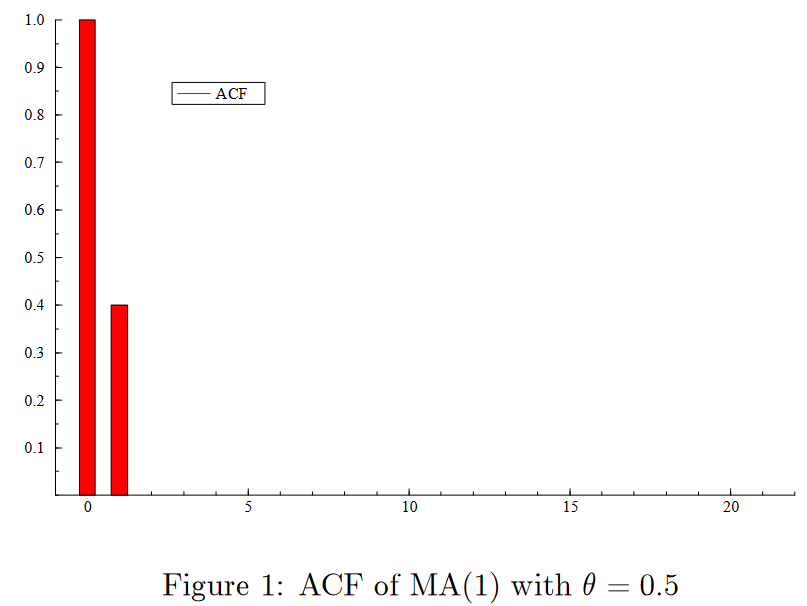
\includegraphics[width=\textwidth]{./Images/MA(1)-ACF.png}
\begin{definition}[Lag operator]
    \[ Ly_t = y_{t-1} \]
    \[ L^{\tau} = y_{t-\tau} \]
\end{definition}
\begin{definition}[Forward operator]
    \[ F y_t = y_{t+1} \]
    \[ F^{\tau} = y_{t+\tau} \]
\end{definition}
\[ L^{-\tau}y_{t+\tau} = F^{\tau} \]
\begin{definition}[First difference operator]
    \[ \Delta = 1-L \]
    Thus $\Delta y_t = y_t - y_{t-1}$
\end{definition}
\begin{definition}[AR(1) Process]
    \[ y_t = \mu + \phi (y_{t-1}-\mu) + \epsilon_t = \delta + \phi y_{t-1} + \epsilon_t \]    
\end{definition}
By weak stationarity when $\phi <1$ we can say $\E [y_t] = \E [y_{t-1}]$. Thus
\[
    \E y_t = \mu + \phi \E y_t - \phi \mu + \E \epsilon_t \implies (1-\phi) \E y_t = (1-\phi) \mu \implies \E y_t = \mu
\]
Further we can say that $Var[y_t] = Var[y_{t-1}]$. Thus
\[
    Var(y_t) = \phi^2 Var(y_t) + Var(\epsilon_t) \implies Var(y_t) = \frac{\sigma^2}{1-\phi^2}
\]
\begin{align*} 
    y_t y_{t-\tau} &= \mu y_{t-\tau} + \phi y_{t-1}y_{t-\tau} - \phi \mu y_{t-\tau} + \epsilon_t y_{t-\tau} \\
    \E[y_t y_{t-\tau}] &= \mu \E[y_{t-\tau}] + \phi \E[y_{t-1}y_{t-\tau}] - \phi \mu \E[y_{t-\tau}] + \E[\epsilon_t y_{t-\tau}] \\
    \E[y_t y_{t-\tau}] - \mu^2 &= \phi ( \E [y_{t-1}y_{t-\tau}] - \mu^2 )\\
    \gamma(\tau) &= \phi \gamma(\tau-1)
\end{align*}
We can solve this first order difference equation to find:
\begin{align*}
    \gamma(\tau) &= \phi \gamma(\tau-1) \\
    &= \phi^2 \gamma(\tau-2) \\
    &= \dots \\
    &= \phi^{\tau} \gamma(0) \\
    &\implies \rho(\tau) = \phi^{\tau}
\end{align*}
Since $|\phi| < 1$, the autocorrelation function is a decreasing exponential function of $\tau$. 
\\
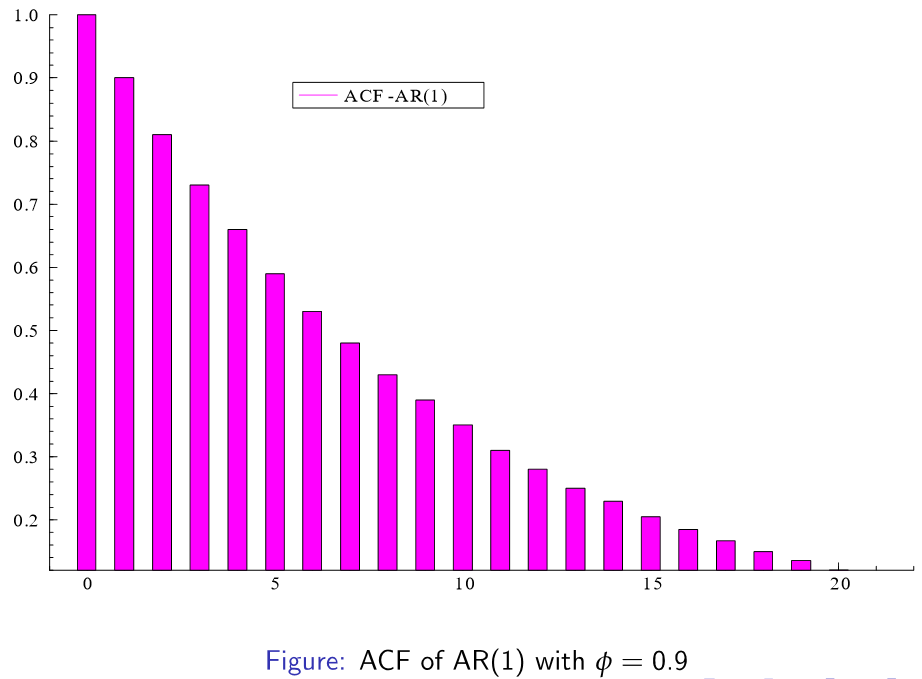
\includegraphics[width=\textwidth]{./Images/AR(1)-ACF.png}
\begin{definition}[Linear process]
A time series is a linear process when it can be expressed as \[
    y_t = \sum_{j= 0}^{\infty} \psi_j \epsilon_{t-j}
    \]
    where $\epsilon_t$ is serially uncorrelated, with mean zero and variance $\sigma^2$, and $\sum_{j=0}^{\infty} |\psi_j| < \infty$. Such a sequence is said to be absolutely convergent.
\end{definition}
A linear process is stationary and its properties may be expressed in terms of the autocovariance function. These properties can be approximated, to any desired level of accuracy, by using an autoregressive-moving average model of order (p,q).
\begin{definition}[ ARMA Process]
\[ y_t = \phi_1 y_{t-1} + \dots + \phi_p y_{t-p} + \theta_1 \epsilon_{t-1} + \dots + \theta_q \epsilon_{t-q} + \epsilon_t \] Also written as $y_t \sim ARMA(p,q)$.
\end{definition}
An ARMA(p,q) can be written more concisely by defining polynomials in the lag operator:
\[
    \phi (L) = 1 - \phi_1 L - \dots - \phi_p L^p\\
    \theta (L) = 1 + \theta_1 L + \dots + \theta_q L^q
\]
Which allows us to express the ARMA as:
\[
    \phi (L) y_t = \theta (L) \epsilon_t
\]

\begin{example}[ARMA(1,1)]
    $y_t = \phi y_{t-1} + \epsilon_t + \theta \epsilon_{t-1}$ \\
    We can write this as $(1-\phi L) y_t = (1 + \theta L) \epsilon_t$ and divide both sides by $1- \phi L$ to get 
    \begin{align*} 
        y_t &= \frac{\epsilon_t}{1-\phi L} + \frac{\theta \epsilon_{t-1}}{1-\phi L} \\
        &= \sum_{j=0}^{\infty} (\phi L)^j \epsilon_t + \theta \sum_{j=0}^{\infty} (\phi L)^j  \epsilon_{t-1} \\
        &= \sum_{j=0}^{\infty} (\phi)^j \epsilon_{t-j} + \theta \sum_{j=0}^{\infty} (\phi)^j  \epsilon_{t-j-1} \\
        &= \epsilon_t + \sum_{j=1}^{\infty} ((\phi)^j + \theta (\phi)^{j-1}) \epsilon_{t-j} \\
        &= \epsilon_t + (\phi + \theta) \sum_{j=1}^{\infty} (\phi)^{j-1} \epsilon_{t-j}
    \end{align*}
    Thus \textbf{we have stationarity if $|\phi| < 1$ }, the weights decline sufficiently rapidly for the process to have finite variance and for the autocovariances to exist.\\
    To derive the autocovariance function, we multiply both sides by $y_{t-\tau}$ and take expectations:
    \begin{align*}
        y_t y_{t-\tau} &= \phi y_{t-1} y_{t-\tau} + \epsilon_t y_{t-\tau} + \theta \epsilon_{t-1} y_{t-\tau} \\
        \E[y_t y_{t-\tau}] &= \phi \E[y_{t-1} y_{t-\tau}] + \E[\epsilon_t y_{t-\tau}] + \theta \E[\epsilon_{t-1} y_{t-\tau}] \\
        \gamma(\tau) &= \phi \gamma(\tau-1) + \E[\epsilon_t y_{t-\tau}] + \theta \E[\epsilon_{t-1} y_{t-\tau}]
    \end{align*}
The last two terms are zero for $\tau >1$. For $\tau = 1$ the first remains zero, but the second becomes 
\[
    \E[\epsilon_{t-1}y_{t-1}] = \E[\epsilon_{t-1}(\phi y_{t-2} + \epsilon_{t-1} + \theta \epsilon_{t-2})] = \phi \E[\epsilon_{t-1}y_{t-2}] + \sigma^2 = \sigma^2
\]
When $\tau = 0$, both expectations are non-zero, and given by $\E[\epsilon_t y_t] = \sigma^2$ and 
\[
    \E [\epsilon_{t-1} y_t] = \E [\epsilon_{t-1} (\phi y_{t-1} + \epsilon_t + \theta \epsilon_{t-1})] = \phi \E [\epsilon_{t-1} y_{t-1}] + \theta \E [\epsilon_{t-1}^2] = \phi \sigma^2 + \theta \sigma^2
\]
Thus we have the autocovariance function:
\begin{align*}
    \gamma(0) &= \phi \gamma(1) + \sigma^2 + \theta \phi \sigma^2 + \theta^2 \sigma^2 \\
    \gamma(1) &= \phi \gamma(0) + \theta \sigma^2 \\
    \gamma(\tau) &= \phi \gamma(\tau-1) \quad \tau > 1
\end{align*}
Solving the the first two equations gives:
\begin{align*}
    \gamma(0) &= \frac{1+\theta^2 + 2 \phi \theta}{1-\phi^2} \sigma^2 \\
    \gamma(1) &= \frac{(1+ \phi \theta)(\phi + \theta)}{1-\phi^2} \sigma^2
\end{align*}
Which gives us the ACF:
\begin{align*}
    \rho(1) = \frac{(1+ \phi \theta)(\phi + \theta)}{1+\theta^2 + 2 \phi \theta}\\
    \rho(\tau) = \phi \rho(\tau-1) \quad \tau > 1
\end{align*}
    The autocorrelations display negative decay for $\tau > 1$, with oscillations when $\phi$ is negative (as in AR(1)). However $\rho(1)$ depends on both $\phi$ and $\theta$, with its sign determined by the sign of $phi + \theta$.
\end {example}
\section{Prediction}
Given a set of observations for $y_t$, $t = 1, \dots, T$, the expected value of $y_{t+\ell}$ conditional on the information at time $t=T$ is
\[
\tilde{y}_{T+\ell|T} = \E[y_{T+\ell}|Y_T] = \E_T [y_{T+\ell}] 
\]
where $Y_T$ is the information set. The conditional expectation is an optimal predictor in the sense that it minimises the mean square error.
\begin{proof}
    The estimation error can be written as:
    \[
        y_{T+\ell} - \hat y_{T+\ell|T} = [y_{T+\ell} - \E_T[y_{T+\ell}]] + [\E_T[y_{T+\ell}] - \hat y_{T+\ell|T}]
    \]
    Since the second term is fixed at T, on squaring this term and taking expectations the cross terms disappear leaving
    \begin{align*}
        MSE(\hat y_{T+\ell|T}) &= \E[(y_{T+\ell} - \E_T[y_{T+\ell}])^2] + \E[(\E_T[y_{T+\ell}] - \hat y_{T+\ell|T})^2]\\
        &= Var(y_{T+\ell}|Y_T)+ [\hat y_{T+\ell|T} - \E(y_{T+\ell}|Y_T)]^2
    \end{align*}
    The dirts term (the conditional variance of $y_{T+\ell}$) does not depend on $\hat y_{T+\ell|T}$. Hence the minimum mean square estimate (MMSE) is given by the conditional mean.
\end{proof}
A predictor is linear if it is a linear combination of past observations. For MSE we use the infinite MA representation. Any such predictor can be written as 
\[
    \hat y_{T+\ell|T} = \sum_{j=0}^{\infty} \psi_t+j^* \epsilon_{T-j}
\]
where the $\psi_j^*$'s are pre-specified weights. The predictor is unbiased in the sense that the unconditional expectation of the predictor 
\[ y_{T+\ell} - \hat y_{T+\ell|T} = \epsilon_{T+\ell} + \psi_1 \epsilon_{T+\ell-1} + \dots + \psi_{\ell-1} \epsilon_{T+1} + (\psi_{\ell}-\psi_{\ell}^*) \epsilon_T + (\psi_{\ell+1} - \psi_{\ell+1}^*) \epsilon_{T-1} + \dots \]
A sufficient condition for ARMA predictions to be linear is that the disturbances are independent (uncorrelatedness not enough).\\
How do we construct an MMSE of a future observation from an ARMA model? We assume the parameters are known and the disturbances are serially independent with mean zero and constant variance $\sigma^2$. An ARMA(p,q) at time $T+\ell$ can be written as
\[
    y_{T+\ell} = \phi_1 y_{T+\ell-1} + \dots + \phi_p y_{T+\ell-p} + \theta_1 \epsilon_{T+\ell-1} + \dots + \theta_q \epsilon_{T+\ell-q} + \epsilon_{T+\ell}
\]
The MMSE of a future observation is its expectation conditional on information at T. Since $\epsilon_t$ are independent they cannot be predicted beyond T, thus have zero conditional expectation. This yields
\[
    \tilde y_{T+\ell|T} = \phi_1 \tilde y_{T+\ell-1|T} + \dots + \phi_p \tilde y_{T+\ell-p|T} + \tilde \epsilon_{T+\ell|T} + \dots + \theta_q \tilde \epsilon_{T+\ell-q|T}
\]
where $\tilde y_{T+j|T} = y_{T+j} $ for $j \leq 0$ and 
\[
\tilde{\epsilon}_{T+j|T} = 
\begin{cases}
0 & \text{if } j > 0 \\
\epsilon_{T+j} & \text{if } j \leq 0
\end{cases}
\]
This provides a recursion for computing optimal predictions of future observations.
\begin{example}[AR(1)]
    For an AR(1) process $\tilde y_{T+\ell|T} = \phi \tilde y_{T+\ell-1|T}$. The starting value is $\tilde y_{T|T} = y_T$. Thus and so 
    \[
        \tilde y_{T+\ell|T} = \phi^{\ell} y_T \quad \ell = 1,2,\dots    
    \]
    The predicted values decline exponentially towards zero; the forecast function has exactly same form as the autocovariance function. This makes sense intuitively: less correlation means less ability to forecast.
\end{example}
\begin{example}[MA(1)]
    For an MA(1) process at time T+1 $y_{T+1} = \epsilon_{T+1} + \theta \epsilon_T$. Thus taking conditional expectations $\tilde y_{T+1|T} = \theta \epsilon_{T}$. For $\ell > 1$ $\tilde y_{T+\ell|T} = 0$ and so the current observation is of no help predicting more than one period ahead.
\end{example}
To find the prediction MSE, we use the infinite MA representation
\[
    y_{T+\ell} = \sum_{j=0}^{\ell -1 } \psi_j \epsilon_{T+\ell-j} + \sum_{j=0}^{\infty} \psi_{\ell+j} \epsilon_{T-j}, \quad IID(0, \sigma^2)
\]
The first term is unknown at t, whilst the second term is known. Taking expectations conditional on $Y_T$ shows that the second term gives an expression for the MMSE of $y_{T+\ell}$:
\[
    \tilde y_{T+\ell|T} = \sum_{j=0}^{\infty} \psi_{\ell+j} \epsilon_{T-j}
\]
Thus the first term of the infinite MA expansion is the error in predicting $\ell$ steps ahead, and its variance is the conditional variance of $y_{T+\ell}$ (which is also the prediction MSE).
\[
    MSE(\tilde y_{T+\ell|T}) = Var_T (y_{T+\ell}) = (1+\psi_1^2 + \dots + \psi_{\ell-1}^2) \sigma^2
\]
\begin{example}
    For the AR(1) process, $\psi_{\ell+ j} = \phi^{\ell+ j}$ and solve\[
        \tilde y_{T+\ell|T} = \sum_{j=0}^{\infty} \phi^{\ell+j} \epsilon_{T-j} = \phi^{\ell} \sum_{j=0}^{\infty} \phi^{j} \epsilon_{T-j} = \phi^{\ell} y_T
    \]
    The MSE is 
    \[
    MSE(\tilde y_{T+\ell|T}) = (1 + \phi^2 + \dots + \phi^{2(\ell-1)}) \sigma^2 = \frac{1-\phi^{2\ell}}{1-\phi^2} \sigma^2
    \]
    As $\ell \to \infty$ the MSE converges to $\sigma^2/(1-\phi^2)$, the unconditional variance of the process. 
\end{example}
Making the additional assumption that the shocks are normal (thus the conditional distribution of $y_{t+\ell}$ is normal), a 95\% confidence interval is given by
\[
    CI(y_{T+\ell})_{0.95} = \tilde y_{T+\ell|T} \pm 1.96\sigma \sqrt{1+\sum_{j=1}^{\ell-1} \psi_j^2} 
\]
\section{Skip sampling and temporal aggregation}
Suppose a model for $y_t^{\dagger}$ is defined for $t = 1,2,\dots, T$ but observations are only available at times $t = \delta, 2\delta, \dots, T$. For example a model may be formulated at the monthly level but observations are only observed quarterly.
\begin{example}
Let $y^\dagger_t$ be an AR(1) model and assume sample size $T/\delta$ is an integer. Then 
\begin{align*}
    y^\dagger_t &= \phi y^\dagger_{t-1} + \epsilon_t \\
    &= = \phi^2 y^\dagger_{t-2} + \phi \epsilon_{t-1} + \epsilon_t \\
    &= \dots \\
    &= \phi^\delta y^\dagger_{t-\delta} + \sum_{j=0}^{\delta-1} \phi^j \epsilon_{t-j}
\end{align*}
The observation model is then:
\begin{align*}
    y_\tau &= \phi^\delta y_{\tau-1} + \sum_{j=0}^{\delta-1} \phi^j \epsilon_{\tau-j}\\
    &\coloneq \phi^\delta y_{\tau-1} + \eta_\tau
\end{align*}
where $y_\tau = y_{\delta \tau}^\dagger$ and $\eta_\tau$ is serially uncorrelated with zero mean and 
\[
    Var(\eta_\tau) = \frac{1-\phi^{2\delta}}{1-\phi^2} 
\]
The observation model is still AR(1) with the same unconditional variance, however the autocorrelations become smaller as $\delta$ increases. 
\end{example}
\begin{question}
    Show that an $MA(q)$ model for $y_t^\dagger$ is WN when $\delta > q$.
\end{question}
\begin{solution}
\[
  y_t^\dagger = \epsilon_t + \sum_{j=1}^{q} \theta_j \epsilon_{t-j} \]
  \[y_{t+\delta}^\dagger = \epsilon_{t+\delta} + \sum_{j=1}^{q} \theta_j \epsilon_{t+\delta-j}\]
When $\delta > q$ the two observations are independent (since there are no common terms); we can write the observation model as
\[
    y_\tau = \eta_\tau 
\]
where $\eta_\tau = \epsilon_t + \sum_{j=1}^{q} \theta_j \epsilon_{t-j}$ which is white noise since the $\epsilon_t$ are independent. Thus
\[
    \eta_\tau \sim WN(0, \sigma^2(1+\theta_1^2 + \dots + \theta_q^2))
\]
\begin{note}
    This result is proved generally in Brewer (1973) who shows that when $y_t^\dagger$ is an ARMA(p,q) process the observation model $y_\tau$ is $ARMA(p, [\delta^{-1}(p(\delta -1) + q]))$ where [] denotes the floor function. As 
    $\delta$ grows the model converges to an $ARMA(p,p)$ process for $q \geq p$ and to an $ARMA(p,p-1)$ process for $q < p$.
\end{note}
\end{solution}
The effect of temporal aggregation when \[
    y_\tau = \sum_{j=0}^{\delta-1} y_{\delta \tau -j}^\dagger
\]
is such that when $y_t^\dagger$ is $ARMA(p,q)$, the corresponding model for $y_\tau$ is $ARMA(p, [\delta^{-1}((p+1)(\delta -1) + q]))$.
\begin{example}
    \textbf{An aggregated AR(1) process is ARMA(1,1)}\\
    PROVE LATER
\end{example}
\section{Tests on Sample Autocorrelations}
The sample autocorrelations are $r(\tau) = c(\tau)/c(0)$ where $c(\tau) = T^{-1}\sum_{t=\tau+1}^{T} (y_t - \bar y)(y_{t-\tau} - \bar y)$ is the sample autocovariance.\\
They are asymptotically normal with mean zero and variance $1/T$ when the observations are independent. DOES THIS NEED PROVING?\\
Deriving this test under the assumption of uncorrelatedness is more difficult, hence tests are based on independence. We run a test on the sample autocorrelation at a particular lag $\tau$ by treating $T^{1/2} r(\tau)$ as a standard normal variate. 
\begin{note}
    A test on a particular sample autocorrelation is only valid if the lag is
    specified in advance. This implies some prior knowledge of the nature of the
    series. For example, with quarterly data a test of the significance of r(4)
    would clearly be relevant. However, seasonality aside, such prior knowledge
    is likely to be the exception rather than the rule, and formal tests on single
    autocorrelations are generally restricted to r(1).
\end{note}
At the 5\% level we reject the null hypothesis of no autocorrelation if $|T^{1/2} r(\tau)| > 1.96$, thus it is common to plot two lines on the sample correlogram at $\pm 2\sqrt{T}$.
\begin{definition}[von Neumann ratio]
  \[
    VNR = \frac{T}{T-1}\left[\frac{\sum_{t=2}^{T} (y_t - y_{t-1})^2}{\sum_{t=1}^{T}(y_t - \bar y)^2} \right]
  \]
    where $\bar y$ is the sample mean.
\end{definition}
\begin{claim}
    \[
        VNR \approx 2[1- r(1)]
    \]
\end{claim}
\begin{proof}
    We first note that $(y_t - y_{t-1})^2 = (y_t - \bar y - (y_{t-1}-\bar y))^2$. Thus
    \begin{align*}
        VNR &= \frac{T}{T-1}\left[\frac{\sum_{t=2}^{T} (y_t - y_{t-1})^2}{\sum_{t=1}^{T}(y_t - \bar y)^2} \right] \\
        &= \frac{T}{T-1}\left[\frac{\sum_{t=2}^{T} (y_t - \bar y)^2 + \sum_{t=2}^{T} (y_{t-1} - \bar y)^2 - 2 \sum_{t=2}^{T} (y_t - \bar y)(y_{t-1} - \bar y)}{\sum_{t=1}^{T}(y_t - \bar y)^2} \right] \\
        &= \frac{T}{T-1}\frac{\sum_{t=1}^T (y_t - \bar y)^2 - (y_1-\bar y)^2 + \sum_{t=1}^{T} (y_{t-1} - \bar y)^2 - (y_T - \bar y)^2 }{\sum_{t=1}^{T}(y_t - \bar y)^2} \\
        &-2 \frac{T}{T-1} \frac{\sum_{t=1}^{T} (y_t - \bar y)(y_{t-1} - \bar y) -(y_1 - \bar y)(y_0-\bar y)}{\sum_{t=1}^{T}(y_t - \bar y)^2} \\
        &= \frac{T}{T-1} \left[ 2 - 2r(1) + \frac{(y_1-\bar y)^2 + (y_T - \bar y)^2+ (y_1 - \bar y)(y_0-\bar y)}{\sum_{t=1}^{T}(y_t - \bar y)^2} \right] \\
        \approx 2[1-r(1)]
    \end{align*}
The approximation arises because of the treatment of the end point. Its effect is negligible in moderate or large samples
\end{proof}
When $y_t \sim NID(0, \sigma^2)$, the small sample distribution of $VNR$ is known. When $r(1)=0$, VNR is approximately equal to two, but as r(1) tends towards one, VNR tends towards zero.
\begin{definition}[Durbin-Watson statistic]
    When a static regression is fitted, the Durbin-Watson statistic is often used to test for serial correlation. It is defined in terms of the residuals as
    \[
        DW = \frac{\sum_{t=2}^{T} (e_t - e_{t-1})^2}{\sum_{t=1}^{T}e_t ^2}
    \]
\end{definition}
\begin{definition}[Portmanteau test statistic]
    \[
        Q(p) = T \sum_{\tau=1}^{p} r(\tau)^2
    \]
\end{definition}
\begin{definition}[Ljung-Box test statistic]
    \[
        Q_{LB}(P) = T(T+2) \sum_{\tau=1}^{p} \frac{r(\tau)^2}{T-\tau}
    \]
\end{definition}
Both of the above are asymptotically distributed as $\chi^2(p)$ when the observations are independent, however the LB test approximates a $\chi^2$ better in finite sample.
\begin{note}
    The choice of P is somewhat arbitrary, when P is large the stat captures potentially high autocorrelations at greater lags, but at the expense of power.
\end{note}
\section{Long memory}
    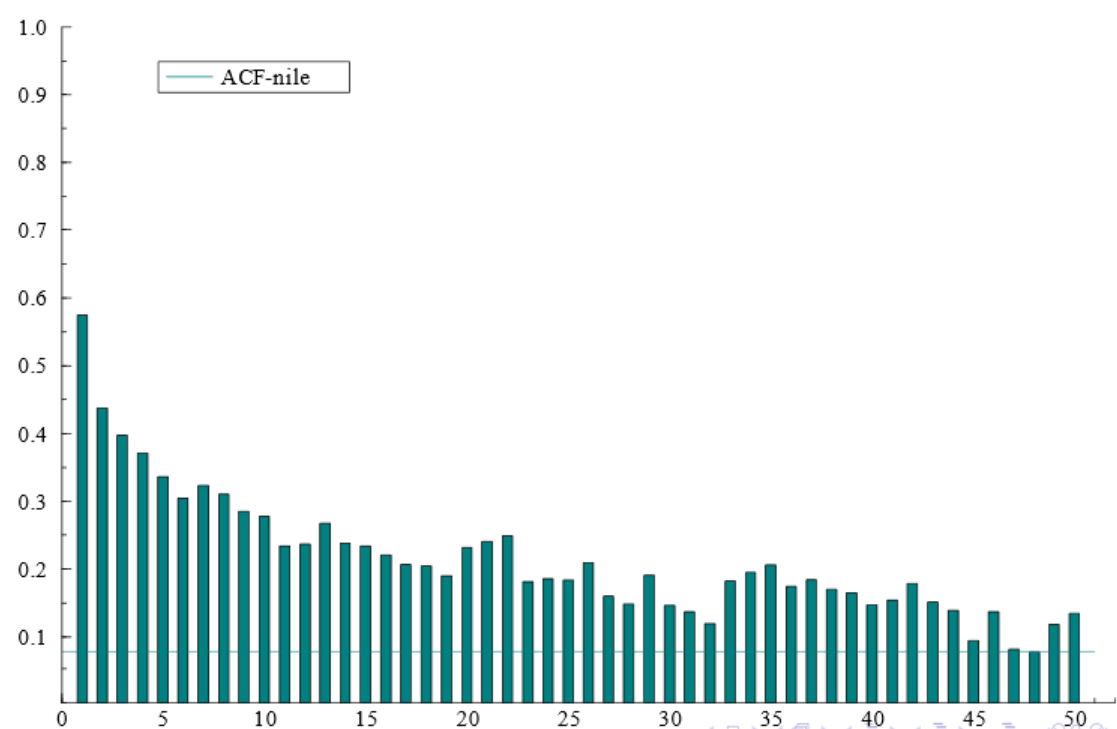
\includegraphics[width=0.5\textwidth]{./Images/Nile-ACF.png}
This is a correlogram of the lowest annual water level of the river Nile (fuck me, bro does not shut up about the Nile). It displays a sharp fall initially followed by a much slower, persistent decline. This pattern is called long memory, which can be produced by a \textbf{fractionally integrated} process.\\
ARIMA(p,d,q) has $(1-L)^d$ generated by an ARMA(p,q), but suppose d is not an integer:
\[
    (1-L)^dy_t = \epsilon_t
\]
where we define the fractional difference operator by the binomial expansion (for any real $d>1$)
\[
    \Delta^d = (1-L)^d = 1-dL-\frac{1}{2}d(1-d)L^2- \cdots
\]
Thus we can write the process in infinite AR form:
\[
    y_t = dy_{t-1} + \frac{1}{2}d(1-d)y_{t-2}+ \dots + \epsilon_t
\]
The coefficients die away very slowly, so a large number of lags is needed to approximate $y_t$ with an AR. We can still use this model for forecasting however.\\
The process is stationary if $d<1/2$. Then
\[
    \rho (\tau) = \frac{\Gamma(1-d)\Gamma(\tau+d)}{\Gamma(d)\Gamma(\tau+1-d)}
\]
\section{Maximum Likelihood}
The joint density can be broken down into a set of one-step ahead predictive distributions by writing 
\[
    p(y;\psi) = \prod_{t=1}^{T}p(y_t|Y_{t-1})
\]
where $Y_{t-1}$ is the information set at time $t-1$ and $p(y_1)$ is interpreted as $p(y_1)$, the unconditional density of $y_1$. For example with $T=3$:
\[
    p(y_3, y_2, y_1) = p(y_3|y_2, y_1)p(y_2|y_1)p(y_1)
\]
The conditional densities are independent of each other, enabling ML to be used in the same way as for independent observations.
\subsection{Autoregressive models}
In the stationary Gaussian AR(1) model (with zero mean), the disturbance of $y_t$, conditional on $y_{t-1}$, is normal with mean $\phi y_{t-1}$ and variance $\sigma^2$. Thus $p(y_t|Y_{t-1})$ is $N(\phi y_{t-1}, \sigma^2)$. The log-likelihood function can thus be derived:
\begin{align*}
p(y_t; \phi, \sigma^2) &= \left(\prod_{t=2}^{T} \frac{1}{\sqrt{2\pi \sigma^2}} \exp \left\{ -\frac{1}{2\sigma^2} (y_t - \phi y_{t-1})^2 \right\} \right)p(y_1)\\
&= \left( \frac{1}{2\pi \sigma^2} \right)^{\frac{T-1}{2}} \exp \left\{ -\frac{1}{2\sigma^2} \sum_{t=2}^{T} (y_t - \phi y_{t-1})^2 \right\} p(y_1) \\
\implies \ln p(y_t; \phi, \sigma^2) &= -\frac{T-1}{2} \ln (2\pi)-\frac{T-1}{2} \ln (\sigma^2) - \frac{1}{2\sigma^2} \sum_{t=2}^{T} (y_t - \phi y_{t-1})^2 + \ln p(y_1)
\end{align*}
The last term is the unconditional distribution of $y_1$, which is normal with mean zero and variance $\sigma^2/(1-\phi^2)$. Thus 
\[
    p(y_1) = \frac{1}{\sqrt{2\pi \sigma^2/(1-\phi^2)}} \exp \left\{ -\frac{y_1^2}{2\sigma^2/(1-\phi^2)}  \right\}
\]
\[
    \implies \ln p(y_1) = -\frac{1}{2} \ln (2\pi) - \frac{1}{2} \ln (\sigma^2) + \frac{1}{2}\ln(1-\phi^2) - \frac{1}{2\sigma^2}(1-\phi^2) y_1^2
\]
Thus
\[
    \ln p(y_t; \phi, \sigma^2) = - \frac{T}{2} \ln (2\pi) - \frac{T}{2} \ln (\sigma^2) - \frac{1}{2}\ln(1-\phi^2) - \frac{1}{2\sigma^2}(1-\phi^2) y_1^2 - \frac{1}{2\sigma^2} \sum_{t=2}^{T} (y_t - \phi y_{t-1})^2
\]
The ML estimator of $\phi$ is not linear because the likelihood function is a cubic equation in $\phi$. On the other hand, if the first observation is treated as though it were fixed, the third and fourth terms can be dropped and T replaced by T-1 in the first two, i.e. we set $p(y_1)=1$:
\[
    \ln p(y_t; \phi, \sigma^2) = - \frac{T-1}{2} \ln (2\pi) - \frac{T-1}{2} \ln (\sigma^2) - \frac{1}{2\sigma^2} \sum_{t=2}^{T} (y_t - \phi y_{t-1})^2
\]
The resulting ML estimator of $\phi$ is then given by a regression of $y_t$ on $y_{t-1}$. Since the first two terms of the above log-likelihood are independent of $\phi$, maximising the likelihood function is equivalent to minimising the sum of squares:
\[
    S(\phi) = \sum_{t=2}^{T} (y_t - \phi y_{t-1})^2
\]
The ML estimator is thus given by 
\[
    \tilde \phi = \frac{\sum_{t=2}^{T} y_t y_{t-1}}{\sum_{t=2}^{T} y_{t-1}^2}
\]
and the variance is estimated by 
\[
    avar(\tilde \phi) = \frac{\tilde \sigma^2}{\sum_{t=2}^{T} y_{t-1}^2}, \quad \text{where } \tilde \sigma^2 = \frac{1}{T} \sum_{t=2}^{T} (y_t - \tilde \phi y_{t-1})^2
\]
\textbf{Asymptotics}\\
\[
    \tilde \phi = \frac{\sum_{t=2}^{T} y_t y_{t-1}}{\sum_{t=2}^{T} y_{t-1}^2} = \frac{\sum_{t=2}^{T} \phi y_{t-1}^2 + \epsilon_t y_{t-1}}{\sum_{t=2}^{T} y_{t-1}^2} = \phi + \frac{\sum_{t=2}^{T} \epsilon_t y_{t-1}}{\sum_{t=2}^{T} y_{t-1}^2}
\]
Thus 
\[
    \sqrt{T}(\tilde \phi - \phi) = \frac{\frac{1}{\sqrt{T}}\sum_{t=2}^{T} \epsilon_t y_{t-1}}{\frac{1}{T} \sum_{t=2}^{T} y_{t-1}^2} \\
\]
Recall that $\E[y_t^2] = Var(y_t) = \sigma^2/(1-\phi^2)$. \textcolor{red}{By some LLN (or by ergodicity?)}
\[
    \frac{1}{T} \sum_{t=2}^{T} y_{t-1}^2 \overset{p}{\to} \frac{\sigma^2}{1-\phi^2}
\]
Furthermore
\[ 
\frac{1}{\sqrt{T}}\sum_{t=2}^{T} \epsilon_t y_{t-1} \overset{d}{\to} N(\E(\epsilon_t y_{t-1}), Var(\epsilon_t y_{t-1})) 
\]
By independence of $\epsilon_t$ across time, $\E[\epsilon_t y_{t-1}] = 0$. Further,
\[
    Var(\epsilon_t y_{t-1}) = \E[\epsilon_t^2 y_{t-1}^2] = \E[\epsilon_t^2] \E[y_{t-1}^2] = \sigma^2 \frac{\sigma^2}{1-\phi^2} = \frac{\sigma^4}{1-\phi^2}
\]
where we can split the expectation because $\epsilon_t$ is independent of $y_{t-1}$. Thus
\[
    \frac{1}{\sqrt{T}}\sum_{t=2}^{T} \epsilon_t y_{t-1} \overset{d}{\to} N(0, \frac{\sigma^4}{1-\phi^2})
\]
Applying the CMT:
\begin{align*}
    \sqrt{T}(\tilde \phi - \phi) &= \frac{\frac{1}{\sqrt{T}}\sum_{t=2}^{T} \epsilon_t y_{t-1}}{\frac{1}{T} \sum_{t=2}^{T} y_{t-1}^2} \\
    &\overset{d}{\to} \frac{N(0, \frac{\sigma^4}{1-\phi^2})}{\frac{\sigma^2}{1-\phi^2}}
    \sim N\left(0, \frac{\sigma^4}{1-\phi^2} \frac{(1-\phi^2)^2}{(\sigma^2)^2}\right)
    \sim N(0, 1-\phi^2)
\end{align*}
In other words, $\tilde \phi$ is asymptotically normal with mean $\phi$ and variance $Avar(\tilde \phi)  = \frac{1-\phi^2}{T}$.
\subsection{Moving Average models}
In the MA(1) model,
\[
    y_t = \epsilon_t + \theta \epsilon_{t-1}, \quad \epsilon_t \sim IID(0, \sigma^2), quad t = 1, \dots, T
\]
the distribution of $y_t$ conditional on the disturbance in the previous period is normal with mean $\theta \epsilon_{t-1}$ and variance $\sigma^2$. The full set of disturbances can be computed as $\epsilon_t = y_t - \theta \epsilon_{t-1}$, however without knowledge of $\epsilon_0$ we compute a set of residuals
\[
    \epsilon_t (\theta;\epsilon_0) = y_t - \theta \epsilon_{t-1}(\theta;\epsilon_0), \quad t = 1, \dots, T
\]
with $\epsilon_0(\theta)$ taken to be fixed at zero. The log likelihood takes the same form as the AR(1), where we seek to minimise a sum of squares:
\[
    S(\theta) = \sum_{t=1}^{T} \epsilon_t^2(\theta;\epsilon_0)
\]
This is known as the \textbf{conditional sum of squares (CSS)} estimator since it is conditional on setting $\epsilon_0 = 0$.\\
The likelihood equations are non-linear because the derivative of $\epsilon_t(\theta;\epsilon_0)$ depends on $\theta$. This is in contrast to the AR(1) model where the derivative of the residual with respect to $\phi$ is $-y_{t-1}$. We thus need a different method to minimise $S(\theta)$.\\
Only one parameter is involved here, so we could just do a grid search over (-1,1). \textcolor{red}{Why do we need to constrain it, if we get something outside (-1,1) we can just use 1/estimate?} However, for more general models this may not be viable, here we use Gauss-Newton iteration. For the MA(1) differentiating the error expression gives 
\[
    \frac{ \partial \epsilon_t(\theta;\epsilon_0)}{\partial \theta} = -\theta \frac{\partial \epsilon_{t-1}(\theta;\epsilon_0)}{\partial \theta} - \epsilon_{t-1}(\theta;\epsilon_0) , \quad t = 1, \dots, T
\]
Because $\epsilon_0(\theta)$ is fixed, it follows that $\frac{\partial \epsilon_0(\theta)}{\partial \theta} = 0$. Thus the derivatives are produced by a recursion running parallel to the computation of the residual set. The algorithm proceeds by updating an estimate of $\theta$, $\hat \theta$, from a regression of $\epsilon_t(\theta;\epsilon_0)$ on $z_t(\hat \theta)= \frac{\partial \epsilon_t(\theta;\epsilon_0)}{\partial \theta}$:
\[
    \theta^*=\hat \theta + \frac{\sum_{t=1}^{T} \epsilon_t(\hat \theta;\epsilon_0) z_t(\hat \theta)}{\sum_{t=1}^{T} z_t(\hat \theta)^2}
\]
\textbf{Asymptotics}\\
Provided the model is both stationary and invertible, the CSS estimator of $\theta$ has the same asymptotic distribution as the (infeasible) estimator based on knowledge of initial disturbances. For the MA(1) model:
\[
   \frac{\partial \epsilon_t}{\partial \theta} = -\theta \frac{\partial \epsilon_{t-1}}{\partial \theta} - \epsilon_{t-1} , \quad t = \dots, -1, 0, 1, \dots, T
\]
By writing $z_t = \frac{\partial \epsilon_t}{\partial \theta}$, it becomes clear we have an AR(1): $z_t = -\theta z_{t-1} - \epsilon_{t-1}$. Hence $\E [z_t^2] = Var(z_t) = \frac{\sigma^2}{1-\theta^2}$ leading to the result that $\tilde \theta$ is asymptotically normal with mean $\theta$ and variance $Avar(\tilde \theta) = \frac{1-\theta^2}{T}$.
\end{document}
